\documentclass[tikz,border=10pt]{standalone}
\usepackage[T1]{fontenc}
\usepackage{helvet}
\renewcommand{\familydefault}{\sfdefault}
\usepackage{tikz}
\usetikzlibrary{arrows.meta,positioning,shapes.multipart,shapes.geometric,fit,backgrounds,calc,shadows}

\definecolor{navy}{HTML}{1F3A5F}
\definecolor{teal}{HTML}{0C6B58}
\definecolor{amber}{HTML}{D9822B}
\definecolor{crimson}{HTML}{B42318}
\definecolor{violet}{HTML}{6B21A8}
\definecolor{sky}{HTML}{2186EB}
\definecolor{slate}{HTML}{486581}
\definecolor{mist}{HTML}{F0F4F8}
\definecolor{line}{HTML}{9FB3C8}

\tikzset{
  >={Stealth[length=2.6mm]},
  box/.style={draw=navy, very thick, rounded corners=3pt, fill=white, align=center,
    inner sep=5pt, font=\small, minimum height=9mm},
  softbox/.style={box, draw=slate, thick, fill=mist},
  layer/.style={draw=line, dashed, rounded corners=6pt, inner sep=7pt},
  layertitle/.style={font=\bfseries\small, text=slate, anchor=north west},
  flow/.style={->, thick, draw=navy},
  dflow/.style={->, thick, draw=slate, dashed},
  lbl/.style={font=\scriptsize, text=slate, fill=white, inner sep=1.5pt},
  umlclass/.style={draw=navy, thick, fill=white, rectangle split, rectangle split parts=3,
    rectangle split part fill={navy!12,white,white}, align=left, font=\scriptsize,
    inner sep=3pt, text width=#1},
  umlclass/.default=38mm,
}

\tikzset{
  term/.style={box, rounded corners=10pt, draw=teal, minimum width=3.6cm, font=\small},
  proc/.style={box, minimum width=5.4cm, font=\small},
  dec/.style={diamond, aspect=2.4, draw=amber, very thick, fill=white, align=center,
    font=\small, inner sep=1pt},
}
\begin{document}
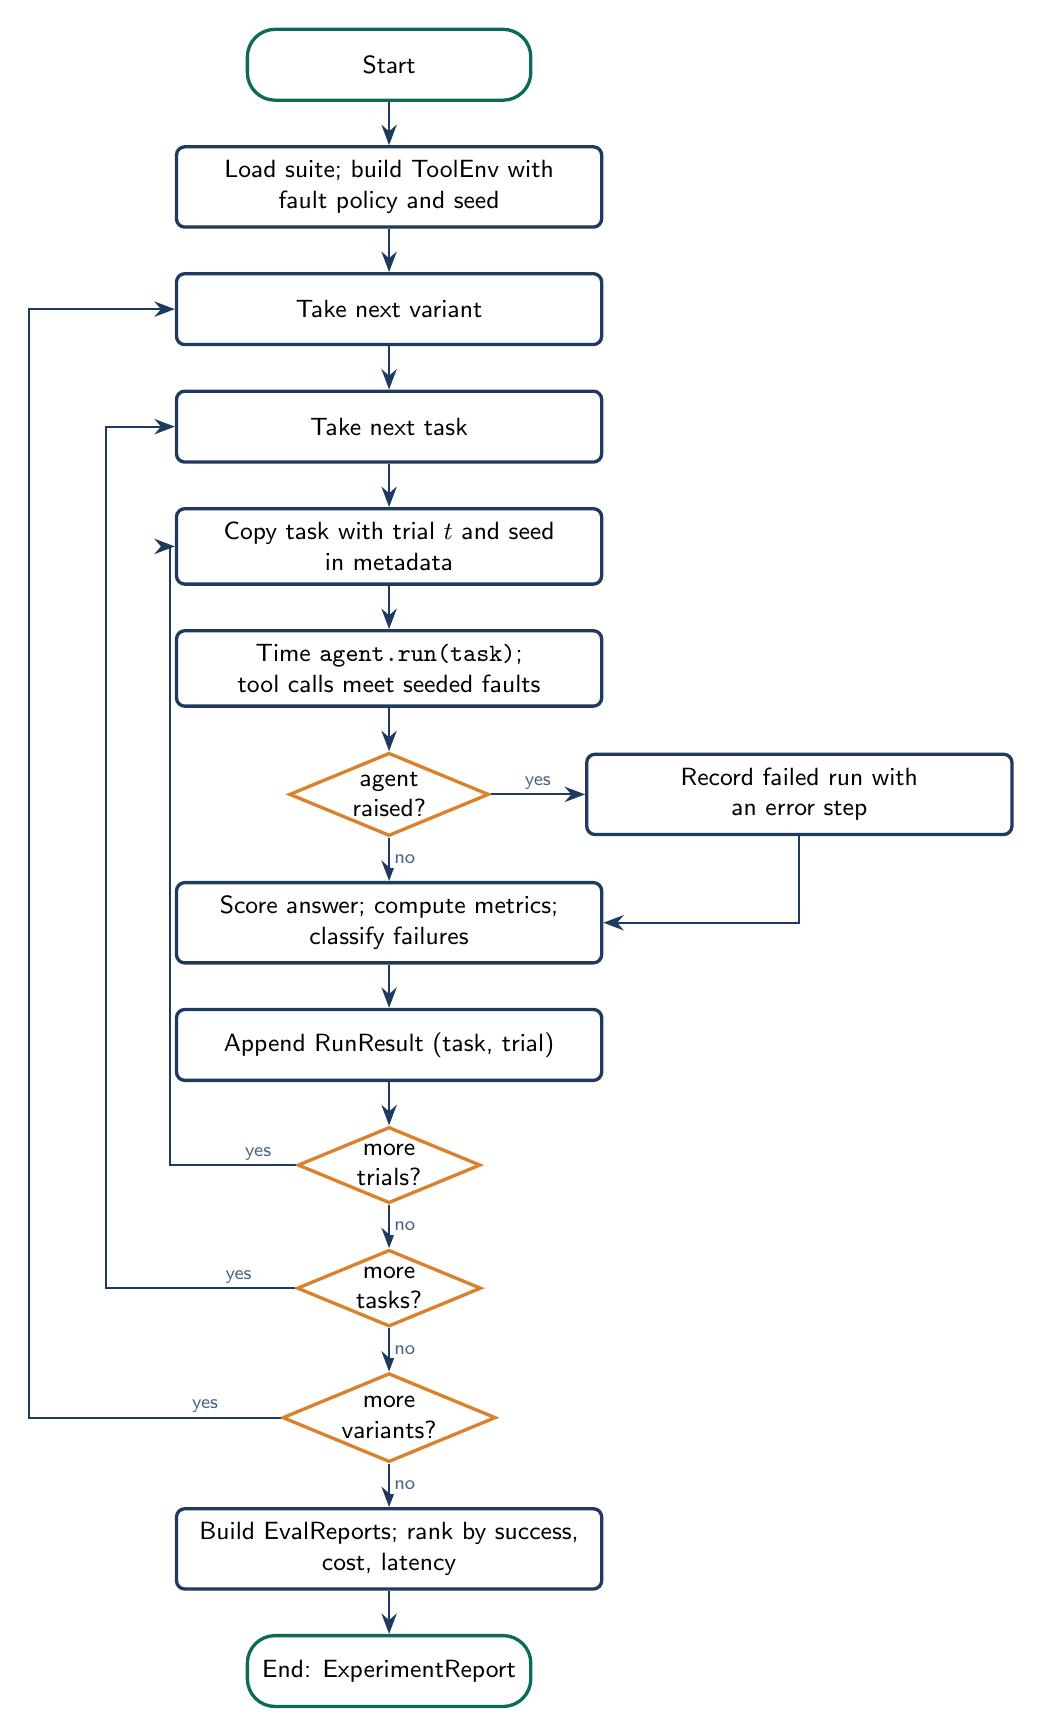
\begin{tikzpicture}[x=1cm,y=1cm, node distance=0.55cm]
  \node[term] (start) {Start};
  \node[proc, below=of start] (load) {Load suite; build ToolEnv with\\ fault policy and seed};
  \node[proc, below=of load] (variant) {Take next variant};
  \node[proc, below=of variant] (task) {Take next task};
  \node[proc, below=of task] (trial) {Copy task with trial $t$ and seed\\ in metadata};
  \node[proc, below=of trial] (runit) {Time \texttt{agent.run(task)};\\ tool calls meet seeded faults};
  \node[dec, below=of runit] (crash) {agent\\ raised?};
  \node[proc, right=1.2cm of crash] (err) {Record failed run with\\ an error step};
  \node[proc, below=of crash] (score) {Score answer; compute metrics;\\ classify failures};
  \node[proc, below=of score] (append) {Append RunResult (task, trial)};
  \node[dec, below=of append] (moretrial) {more\\ trials?};
  \node[dec, below=of moretrial] (moretask) {more\\ tasks?};
  \node[dec, below=of moretask] (morevar) {more\\ variants?};
  \node[proc, below=of morevar] (rank) {Build EvalReports; rank by success,\\ cost, latency};
  \node[term, below=of rank] (stop) {End: ExperimentReport};

  \draw[flow] (start) -- (load);
  \draw[flow] (load) -- (variant);
  \draw[flow] (variant) -- (task);
  \draw[flow] (task) -- (trial);
  \draw[flow] (trial) -- (runit);
  \draw[flow] (runit) -- (crash);
  \draw[flow] (crash) -- node[lbl, above] {yes} (err);
  \draw[flow] (err) |- (score.east);
  \draw[flow] (crash) -- node[lbl, right] {no} (score);
  \draw[flow] (score) -- (append);
  \draw[flow] (append) -- (moretrial);
  \draw[flow] (moretrial.west) -- node[lbl, above, pos=0.3] {yes} ++(-1.6,0) |- (trial.west);
  \draw[flow] (moretrial) -- node[lbl, right] {no} (moretask);
  \draw[flow] (moretask.west) -- node[lbl, above, pos=0.3] {yes} ++(-2.4,0) |- (task.west);
  \draw[flow] (moretask) -- node[lbl, right] {no} (morevar);
  \draw[flow] (morevar.west) -- node[lbl, above, pos=0.3] {yes} ++(-3.2,0) |- (variant.west);
  \draw[flow] (morevar) -- node[lbl, right] {no} (rank);
  \draw[flow] (rank) -- (stop);
\end{tikzpicture}
\end{document}
